\documentclass[a4paper,10pt]{article}
%\documentclass[a4paper,10pt]{scrartcl}

\usepackage[utf8]{inputenc}
\usepackage{graphicx} 
\graphicspath{{.}}

\title{Capital Volume 1}
\author{Charbel Daher}
\date{January 1 2022}

\pdfinfo{%
  /Title    (Capital volume 1)
  /Author   (karl marx)
  /Creator  (rosetorte)
  /Producer ()
  /Subject  (political economy)
  /Keywords (marxism, marx, communism, political economy, socialism)
}

\begin{document}
\maketitle
\tableofcontents
\newpage

\section*{\centering{Book I: The process of production of capital}} 
\section*{\centering{Part one}}
\section{\centering{Chapter 1: The Commodity}}
\subsection{\centering{Section 1: The two factors of a commodity Use-Value and Value (The Substance of Value and the
Magnitude of Value)}}

An economy with a capitalist mode of production produces commodities, ``The wealth of societies in which the capitalist mode
of production prevails appears as an 'immense collection of commodities'". ``A commodity is an external object which
through its qualities satisfies human needs of whatever kind. The nature of these needs whether they arise from the stomach,
or the imagination makes no difference." A use-value of a commodity is the qualitative aspect of a given product, its
utility. For example, a hammer's general utility is to hammer nails. Use values are only realized in consumption, a use-value
is independent from the social nature of a commodity. As soon as a commodity enters a market it now has an Exchange-value. An
exchange-value is the exchange of one kind of use-value for another. Exchange value is the quantitative aspect of a
commodity. For example, how many hammers would I need to exchange for a screwdriver? That relation is a quantitative one.
\[xHammer = yScrewdriver\] this relation shows a common element in which we can equate a number of hammers to a number of
screwdrivers, this is an exchange relation. As we said, this relation is independent of the qualitative aspects of both
commodities that are being exchanged, it is independent of their use-values. Therefore the common element that we use to equate
those two commodities is not a physical aspect of the commodities, but the abstraction of human labour. So what remains is
the value of those commodities, and the value of a commodity is the amount of socially necessary labour required to produce
this product. The magnitude of value is measured by the quantity of value forming substance, the labour, in the commodity.
This quantity is measured by labour-time, the time necessary to preform the labour necessary to produce this commodity (days,
weeks, months...etc). We use the term socially necessary labour-time\footnote{``Socially necessary labour-time" is the same as
``the amount of socially necessary labor".} to denote the average labour-time under normal
production conditions necessary to produce a commodity. Marx gives this example to explain the importance of socially
necessary labour-time: ``The introduction of power-looms into England, for example, probably reduced by one half the labour
required to convert a given quantity of yarn into woven fabric. In order to do this, the English hand-loom weaver in fact
needed the same amount of labour-time as before; but the product of his individual hour of labour now only represented half
an hour of social labour, and consequently fell to one half its former value."  

\newpage
\subsection{\centering{Section 2: The twofold character of labour embodied in commodities}}

As we saw in the first section, the commodity is an object with a dual character, namely Use-value and Exchange-value. What
Marx pointed out is that Labour also has a twofold character. Useful labour is labour whose utility is represented by the
use-value of its product. In a society whose products assume the form of commodities, there has to be a social division of
labour. The labour done by weaving and the labour done by tailoring are two qualitatively different forms of Useful labour,
they produce different Use-values. Two commodities with qualitatively different use-values were produced by different forms
of useful labour. This variation in the forms of labour and use-values of commodities necessitates a social division of
labour. The social division of labour is necessary for commodity production, but the converse does not hold, commodity
production isn't necessary for the social division of labour. Useful labour, as Marx argues, is independent of all forms of
society, it is an eternal necessity in which Man shapes the material products of nature to his own utility. Therefore, if we
subtract the different forms of useful labour from a commodity, its material substratum is always left. For example, a
carpenter might repurpose a branch from a wooden tree to make himself a shovel. This Useful labour is one fold of the twofold
character of labour, it is its qualitative side. The other half of labour is its quantitative side, the unit of simple labour
power is used to measure the magnitude of value. Simple labour power is the amount of labour it takes an average person
within a society to create a use-value. Complex labour is intensified simple labour. This analogy can be made clear by taking
any example of an expert, say a doctor, who would charge more for his time than an average person with no expertise in that
area. The doctor charges more because he takes into account the labour time it took him to become a doctor, the
intensification of average labour power to complex labour, becoming a doctor.
\begin{figure}[!h]
  \centering
  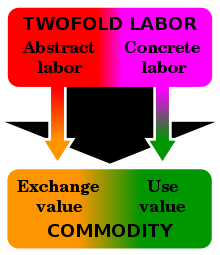
\includegraphics[width=0.27\linewidth]{./images/twofoldlabour.png}
  \caption{The twofold character of Labour}
  \label{fig 1}
\end{figure}
To show clearly the antagagonistic character of labour, you can think of it in this way: The labour necessary to create a
commodity will always remain constant, but the labour-time needed to express that labour is what makes a difference. A worker
can create 2 coats in the same time it takes another worker to create 1 coat, the first worker now produces more use-values,
this is an increase in material wealth. This increase in the productivity of the first labourer is at the expense of the
value of a coat, as now it takes less labour-time to make a coat, its value diminishes.  



\end{document}
